%% 1 row - IPF
\begin{figure}[H]
\centering
      \begin{subfigure}[t]{0.48\textwidth}
        \centering
        \begin{tikzpicture}[scale=1, baseline]
                \begin{customlegend}[legend columns=1,legend style={font=\tiny, column sep=2ex},
                legend entries={Eagle/Intel\textregistered\ Xeon\textregistered\ E5-2697 v3,
                                ARM Hi1616,
                                Intel\textregistered\ Xeon\textregistered\ Gold 6140,
                                AMD Epyc 7551,
                                Power8+ S822LC
                                }]
                \addlegendimage{mark=otimes,solid}
                \addlegendimage{mark=square,solid}
                \addlegendimage{mark=*,solid}
                \addlegendimage{mark=star,solid}
                \addlegendimage{mark=|,solid}
                \end{customlegend}
            \end{tikzpicture}
       \end{subfigure}\hfill
    \begin{subfigure}[t]{0.48\textwidth}
     \centering
        \begin{tikzpicture}[scale=1, baseline]
                \begin{customlegend}[legend columns=1,legend style={font=\tiny, column sep=2ex},
                legend entries={Execution time ,
                                Memory use,
                                No. of system file inputs,
                                No. of system file outputs
                                }]
                \addlegendimage{mark=*,solid}
                \addlegendimage{mark=square,solid}
                \addlegendimage{mark=star,solid}
                \addlegendimage{mark=otimes,solid}
                \end{customlegend}
            \end{tikzpicture}
    \end{subfigure}\bigbreak
    \begin{subfigure}[t]{0.48\textwidth}
        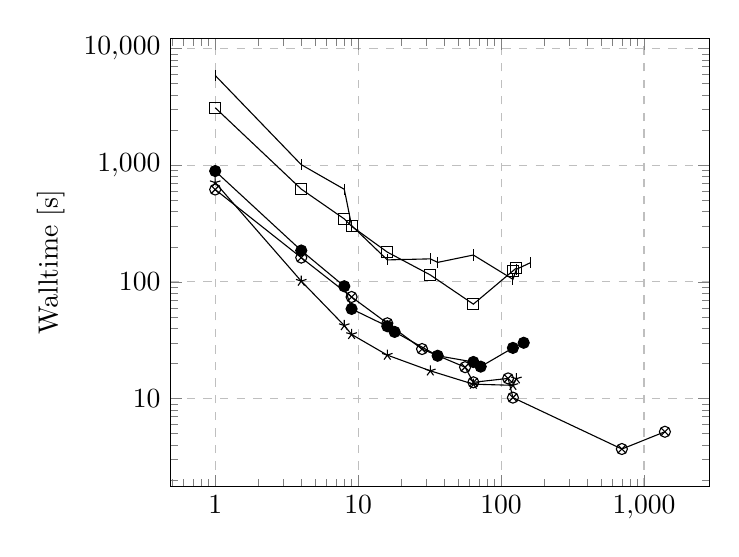
\begin{tikzpicture}[scale=1, baseline]
            \begin{axis}[
            xmode=log,
            ymode=log,
            log ticks with fixed point,
            scaled y ticks=real:1e3
            axis lines = left,
            %xlabel = \#MPI ranks,
            ylabel = {Walltime [s]},
            legend style={at={(0.5,-0.2)},
            	    anchor=north,legend columns=1},
            xmajorgrids=true,
            ymajorgrids=true,
            grid style=dashed,
            ]
                %ARM
                \addplot [
                    domain=1:150, 
                    color=black,
                    mark=square,
                    ]
                    coordinates {                 (1,3107.3)(4,624.3)(8,346.5)(9,299.7)(16,180.1)(32,114.7)(64,64.5)(121,124.3)(128,131.5)};
%                \addlegendentry{ARM Hi1616}
                %Intel 6140
                \addplot [
                    domain=1:150, 
                    color=black,
                    mark=*,
                ]
                coordinates {                   (1,891.2)(4,185.8)(8,91.8)(9,58.7)(16,41.7)(18,37.3)(36,23.3)(64,20.6)(72,18.8)(121,27.2)(144,30.1)};
%                \addlegendentry{Intel\textregistered\ Xeon\textregistered\ Gold 6140}
                %AMD Epyc
                \addplot [
                    domain=1:150, 
                    color=black,
                    mark=star,
                    ]
                    coordinates {
                   (1,709.9)(4,101.6)(8,42.3)(9,35.5)(16,23.6)(32,17.3)(64,13.3)(121,13.0)(128,14.8)};
 %               \addlegendentry{AMD Epyc 7551}
                %Eagle
                \addplot [
                    domain=1:1400, 
                    color=black,
                    mark=otimes,
                    ]
                    coordinates {                    (1,618.9)(4,161.5)(9,74.3)(16,44.2)(28,26.6)(56,18.6)(64,13.8)(112,14.9)(121,10.2)(700,3.7)(1400,5.2)
                    };
%               \addlegendentry{Eagle/Intel\textregistered\ Xeon\textregistered\ E5-2697 v3}
                %Power
                \addplot [
                    domain=1:150, 
                    color=black,
                    mark=|,
                    ]
                    coordinates {
                    (1,5878.0)(4,1010.5)(8,621.8)(9,304.1)(16,154.4)(32,157.6)(36,147)(64,170)(121,105.3)(128,128.3)(160,145.8)
                    };
%                \addlegendentry{Power8+ S822LC}
            \end{axis}
        \end{tikzpicture}
        \caption{IPF scalability}
        \label{fig:ipf_scalability}
    \end{subfigure}\hfill
    \begin{subfigure}[t]{0.48\textwidth}
        \centering
        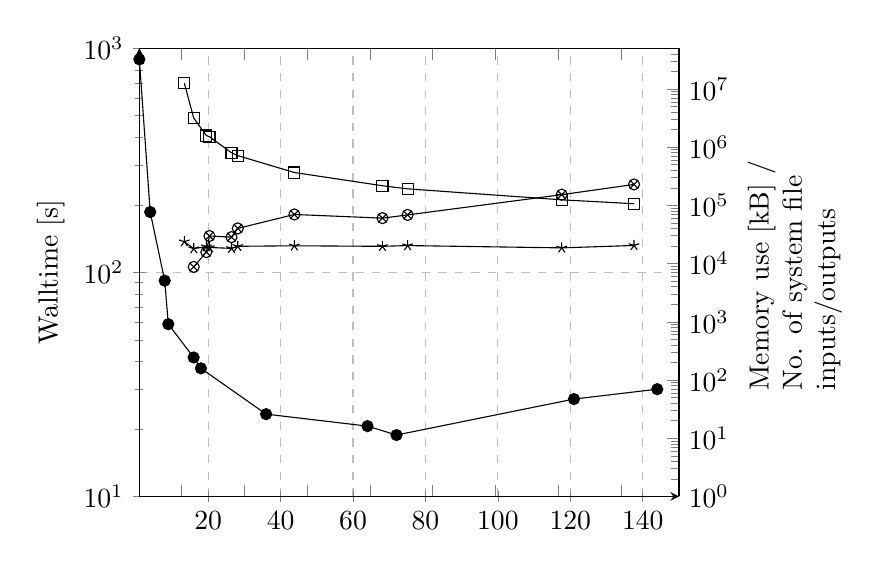
\begin{tikzpicture}[scale=1, baseline]
            \begin{axis}[
            %    width=1\textwidth,
                axis y line*=left,
                axis lines = left,
                %%xlabel = \#MPI ranks,
                ylabel = {Walltime [s]},
                xmajorgrids=true,
                ymajorgrids=true,
                grid style=dashed,
                xmin=1, xmax=150,
                ymode=log,
                ymin=10, ymax=1000,
                ]
                %Execution time
                \addplot [
                    domain=1:70, 
                    color=black,
                    mark=*,
                ]
                coordinates {                   (1,891.2)(4,185.8)(8,91.8)(9,58.7)(16,41.7)(18,37.3)(36,23.3)(64,20.6)(72,18.8)(121,27.2)(144,30.1)};
                \label{ipf_execution_time}
            \end{axis}
            \begin{axis}[
%                xmode=log,
                ymode=log,
                xticklabel=\empty,
                axis y line*=right,
                scaled ticks=false,
                y tick label style={/pgf/number format/.cd,sci,sci e},
                ymin=1, ymax=50000000,
                ylabel style={text width=3cm},
                ylabel = {Memory use {[kB]} {/} No. of system file inputs/outputs},
                legend style={at={(0.5,-0.2)},
                	    anchor=north,legend columns=1},
                grid style=dashed,
                ]
                \addlegendimage{/pgfplots/refstyle=ipf_execution_time}
%                \addlegendentry{Execution time}
                %RAM
                \addplot [
                    domain=1:70, 
                    color=black,
                    mark=square,
                    ]
                    coordinates {(1,12510916)(4,3140960)(8,1579868)(9,1505996)(16,800212)(18,713344)(36,365920)(64,216960)(72,191912)(121,124292)(144,106468)};
%                \addlegendentry{Memory use}
                %#inputs
                \addplot [
                    domain=1:70, 
                    color=black,
                    mark=star,
                    ]
                    coordinates {(1,23752)(4,18024)(8,19488)(9,18888)(16,18224)(18,19792)(36,20192)(64,19768)(72,20368)(121,18592)(144,20464)};
  %              \addlegendentry{No. of system file inputs}
                %#outputs
                \addplot [
                    color=black,
                    mark=otimes,
                    ]
                    coordinates {(1,0)(4,8760)(8,15728)(9,29744)(16,28400)(18,40128)(36,69664)(64,60248)(72,68416)(121,152384)(144,228360)};
 %                   \addlegendentry{No. of system file outputs}
            \end{axis}
            \end{tikzpicture}
          \caption{IPF on Intel\textregistered\ Xeon\textregistered\ Gold 6140}
          \label{fig:ipf_intel_gold}
      \end{subfigure}\bigbreak
%      \caption{Results for IPF}
%\end{figure}

%% 2 row - Pandora/GG
%\begin{figure}[ht]
%\centering
    \begin{subfigure}[t]{0.48\textwidth}
        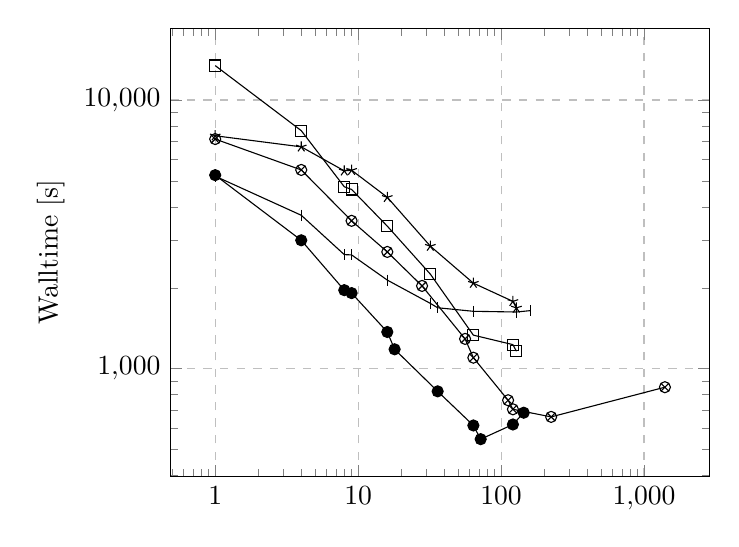
\begin{tikzpicture}[scale=1, baseline]
            \begin{axis}[
            xmode=log,
            ymode=log,
            log ticks with fixed point,
            scaled y ticks=real:1e3
            axis lines = left,
            %xlabel = \#MPI ranks,
            ylabel = {Walltime [s]},
%            legend style={at={(0.5,-0.2)},
%            	    anchor=north,legend columns=1},
            xmajorgrids=true,
            ymajorgrids=true,
            grid style=dashed,
            ]
                %ARM
                \addplot [
                    domain=1:150, 
                    color=black,
                    mark=square,
                    ]
                    coordinates {                 (1,13437.4)(4,7694.2)(8,4756.2)(9,4647.5)(16,3393.4)(32,2249)(64,1333.4)(121,1229.1)(128,1161.9)};
%                \addlegendentry{ARM Hi1616}
                %Intel 6140
                \addplot [
                    domain=1:150, 
                    color=black,
                    mark=*,
                ]
                coordinates {                   (1,5253.9)(4,3005.9)(8,1960.8)(9,1911.8)(16,1369.7)(18,1180.8)(36,823.6)(64,614.9)(72,546.6)(121,620.0)(144,685.8)};
%                \addlegendentry{Intel\textregistered\ Xeon\textregistered\ Gold 6140}
                %AMD Epyc
                \addplot [
                    domain=1:150, 
                    color=black,
                    mark=star,
                    ]
                    coordinates {
                   (1,7364.1)(4,6696.0)(8,5451.3)(9,5480)(16,4345.6)(32,2859.2)(64,2081.9)(121,1781.2)(128,1683.8)};
 %               \addlegendentry{AMD Epyc 7551}
                %Eagle
                \addplot [
                    domain=1:1400, 
                    color=black,
                    mark=otimes,
                    ]
                    coordinates {                    (1,7158.7)(4,5493.6)(9,3552.1)(16,2720.5)(28,2033)(56,1291.2)(64,1099.1)(112,763.1)(121,706.3)(224,661.7)(1400,853.4)
                    };
%                \addlegendentry{Eagle/Intel\textregistered\ Xeon\textregistered\ E5-2697 v3}
                %Power
                \addplot [
                    domain=1:150, 
                    color=black,
                    mark=|,
                    ]
                    coordinates {
                    (1,5208.5)(4,3725.4)(8,2658.6)(9,2652.2)(16,2137.1)(32,1750.5)(36,1686.2)(64,1635.6)(128,1625.7)(160,1644.8)
                    };
%                \addlegendentry{Power8+ S822LC}
            \end{axis}
        \end{tikzpicture}
        \caption{Pandora/GG scalability (WW map)}
        \label{fig:pandora_scalability}
    \end{subfigure}\hfill
    \begin{subfigure}[t]{0.48\textwidth}
        \centering
        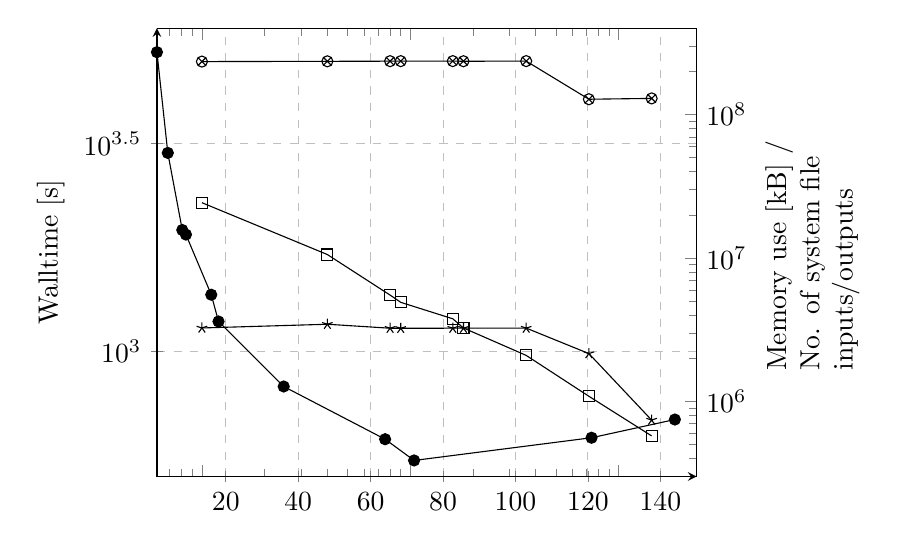
\begin{tikzpicture}[scale=1, baseline]
            \begin{axis}[
            %    width=1\textwidth,
                axis y line*=left,
                axis lines = left,
                %xlabel = \#MPI ranks,
                ylabel = {Walltime [s]},
                xmajorgrids=true,
                ymajorgrids=true,
                grid style=dashed,
                xmin=1, xmax=150,
                ymode=log,
                ymin=500, ymax=6000,
                ]
                %Execution time
                \addplot [
                    domain=1:70, 
                    color=black,
                    mark=*,
                ]
                coordinates {                   (1,5253.9)(4,3005.9)(8,1960.8)(9,1911.8)(16,1369.7)(18,1180.8)(36,823.6)(64,614.9)(72,546.6)(121,620.0)(144,685.8)};
                \label{pandora_execution_time}
            \end{axis}
            \begin{axis}[
                xmode=log,
                ymode=log,
                xticklabel=\empty,
                axis y line*=right,
                scaled ticks=false,
                y tick label style={/pgf/number format/.cd,sci,sci e},
                ymin=300000, ymax=400000000,
                ylabel style={text width=3cm},
                ylabel = {Memory use {[kB]} {/} No. of system file inputs/outputs},
                legend style={at={(0.5,-0.2)},
                	    anchor=north,legend columns=1},
                grid style=dashed,
                ]
                \addlegendimage{/pgfplots/refstyle=pandora_execution_time}
%                \addlegendentry{Execution time}
                %RAM
                \addplot [
                    domain=1:70, 
                    color=black,
                    mark=square,
                    ]
                    coordinates {(1,24316736)(4,10578468)(8,5519380)(9,4912336)(16,3772628)(18,3255200)(36,2096424)(72,1087508)(144,575948)};
 %               \addlegendentry{Memory use}
                %#inputs
                \addplot [
                    domain=1:70, 
                    color=black,
                    mark=star,
                    ]
                    coordinates {(1,3255992)(4,3455808)(8,3243280)(9,3237968)(16,3245208)(18,3244448)(36,3249248)(72,2158432)(144,742416)};
 %               \addlegendentry{No. of system file inputs}
                %#outputs
                \addplot [
                    color=black,
                    mark=otimes,
                    ]
                    coordinates {(1,234115384)(4,235057696)(8,235684024)(9,235765544)(16,235883464)(18,235413696)(36,235913920)(72,127931040)(144,129657720)};
%                    \addlegendentry{No. of system file outputs}
            \end{axis}
            \end{tikzpicture}
          \caption{Pandora/GG on Intel\textregistered\ Xeon\textregistered\ Gold 6140}
          \label{fig:pandora_intel_gold}
      \end{subfigure}\bigbreak
%      \caption{Results for Pandora/GG (worldwide map)}
%\end{figure}



%% 3 row - ABMS4py
%\begin{figure}[ht]
%\centering
    \begin{subfigure}[t]{0.48\textwidth}
        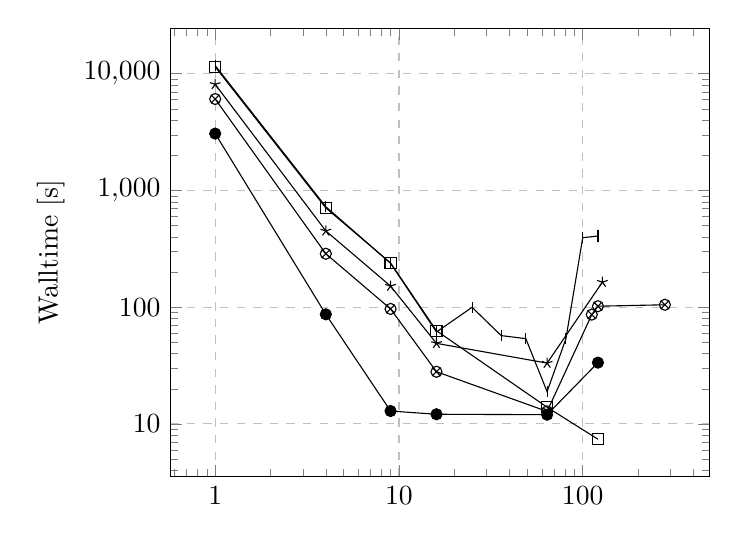
\begin{tikzpicture}[scale=1, baseline]
            \begin{axis}[
            xmode=log,
            ymode=log,
            log ticks with fixed point,
            scaled y ticks=real:1e3
            axis lines = left,
            %xlabel = \#MPI ranks,
            ylabel = {Walltime [s]},
%            legend style={at={(0.5,-0.2)},
%            	    anchor=north,legend columns=1},
            xmajorgrids=true,
            ymajorgrids=true,
            grid style=dashed,
            ]
                %ARM
                \addplot [
                    domain=1:150, 
                    color=black,
                    mark=square,
                    ]
                    coordinates {                 (1,11463.3)(4,708.9)(9,239.5)(16,62.9)(64,13.9)(121,7.4)};
%                \addlegendentry{ARM Hi1616}
                %Intel 6140
                \addplot [
                    domain=1:150, 
                    color=black,
                    mark=*,
                ]
                coordinates {                   (1,3071.5)(4,86.9)(9,12.9)(16,12.1)(64,12.0)(121,33.5)};
%                \addlegendentry{Intel\textregistered\ Xeon\textregistered\ Gold 6140}
                %AMD Epyc
                \addplot [
                    domain=1:150, 
                    color=black,
                    mark=star,
                    ]
                    coordinates {
                   (1,8114.8)(4,450.3)(9,151.7)(16,49.0)(64,33.2)(128,164)};
%                \addlegendentry{AMD Epyc 7551}
                %Eagle
                \addplot [
                    domain=1:1400, 
                    color=black,
                    mark=otimes,
                    ]
                    coordinates {                    (1,6077.3)(4,287)(9,96.7)(16,28)(64,12.8)(112,86.4)(121,102)(280,104.9)
                    };
%                \addlegendentry{Eagle/Intel\textregistered\ Xeon\textregistered\ E5-2697 v3}
                %Power
                \addplot [
                    domain=1:150, 
                    color=black,
                    mark=|,
                    ]
                    coordinates {
                    (1,11751.7)(4,725.9)(9,237.9)(16,61.3)(25,99.8)(36,57.1)(49,53.8)(64,18.9)(81,53.7)(100,394.1)(121,407.3)
                    };
%                \addlegendentry{Power8+ S822LC}
            \end{axis}
        \end{tikzpicture}
        \caption{ABMS4py scalability}
        \label{fig:abms_scalability}
    \end{subfigure}\hfill
    \begin{subfigure}[t]{0.48\textwidth}
        \centering
        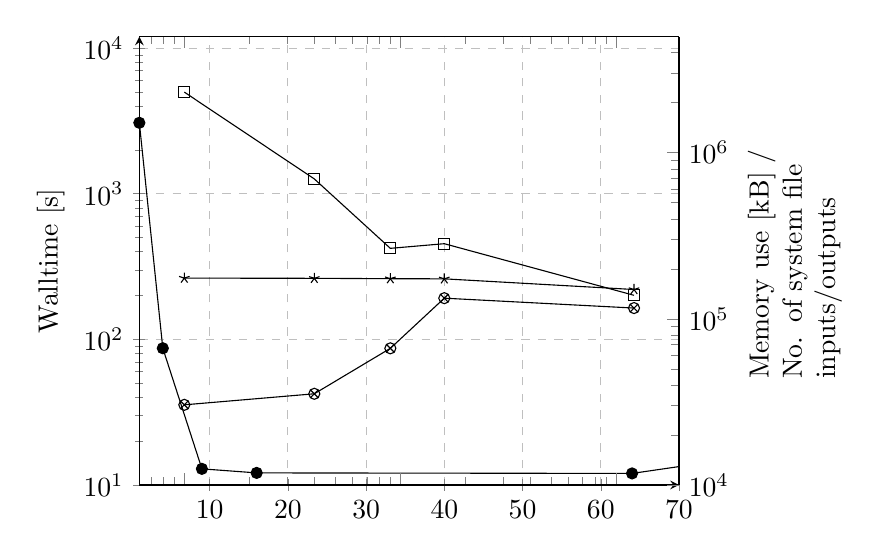
\begin{tikzpicture}[scale=1, baseline]
            \begin{axis}[
            %    width=1\textwidth,
                axis y line*=left,
                axis lines = left,
                %xlabel = \#MPI ranks,
                ylabel = {Walltime [s]},
                xmajorgrids=true,
                ymajorgrids=true,
                grid style=dashed,
                xmin=1, xmax=70,
                ymode=log,
                ymin=10, ymax=12000,
                ]
                %Execution time
                \addplot [
                    domain=1:70, 
                    color=black,
                    mark=*,
                ]
                coordinates {                   (1,3071.5)(4,86.9)(9,12.9)(16,12.1)(64,12.0)(121,33.5)};
                \label{abms_execution_time}
            \end{axis}
            \begin{axis}[
                xmode=log,
                ymode=log,
                xticklabel=\empty,
                axis y line*=right,
                scaled ticks=false,
                y tick label style={/pgf/number format/.cd,sci,sci e},
                ymin=10000, ymax=5000000,
                ylabel style={text width=3cm},
                ylabel = {Memory use {[kB]} {/} No. of system file inputs/outputs},
%                legend style={at={(0.5,-0.2)},
%                	    anchor=north,legend columns=1},
                grid style=dashed,
                ]
                \addlegendimage{/pgfplots/refstyle=abms_execution_time}
%                \addlegendentry{Execution time}
                %RAM
                \addplot [
                    domain=1:70, 
                    color=black,
                    mark=square,
                    ]
                    coordinates {(1,2316696)(4,695464)(9,265676)(16,283352)(121,138564)};
%              \addlegendentry{Memory use}
                %#inputs
                \addplot [
                    domain=1:70, 
                    color=black,
                    mark=star,
                    ]
                   coordinates {(1,175888)(4,175368)(9,174456)(16,174088)(121,150160)};
%               \addlegendentry{No. of system file inputs}
                %#outputs
                \addplot [
                    color=black,
                    mark=otimes,
                    ]
                    coordinates {(1,30360)(4,35384)(9,66448)(16,133160)(121,116104)};
%                    \addlegendentry{No. of system file outputs}
            \end{axis}
            \end{tikzpicture}
          \caption{ABMS4py Intel\textregistered\ Xeon\textregistered\ Gold 6140}
          \label{fig:abms_intel_gold}
      \end{subfigure}\bigbreak
      \caption{Results for social simulation applications}
\end{figure}
